\documentclass[onecolumn, draftclsnofoot,10pt, compsoc]{IEEEtran}
\usepackage{graphicx}
\usepackage{url}
\usepackage{setspace}

\usepackage{geometry}
\geometry{textheight=9.5in, textwidth=7in}

\def \CapstoneTeamNumber{55}
\def \GroupMemberOne{Riley Rimer}
\def \GroupMemberTwo{River Hendriksen}
\def \GroupMemberThree{Corey Hemphill}
\def \CapstoneProjectName{CoverageJSON Response Handler for OPeNDAP}
\def \CapstoneSponsorCompany{NASA Jet Propulsion Laboratory}
\def \CapstoneSponsorPerson{Lewis John McGibbney}

\def \DocType{	%Problem Statement
				Requirements Document
				%Technology Review
				%Design Document
				%Progress Report
				}
			
\newcommand{\NameSigPair}[1]{\par
\makebox[2.75in][r]{#1} \hfil 	\makebox[3.25in]{\makebox[2.25in]{\hrulefill} \hfill		\makebox[.75in]{\hrulefill}}
\par\vspace{-12pt} \textit{\tiny\noindent
\makebox[2.75in]{} \hfil		\makebox[3.25in]{\makebox[2.25in][r]{Signature} \hfill	\makebox[.75in][r]{Date}}}}
% 3. If the document is not to be signed, uncomment the RENEWcommand below
\renewcommand{\NameSigPair}[1]{#1}

%%%%%%%%%%%%%%%%%%%%%%%%%%%%%%%%%%%%%%%
\begin{document}
\begin{titlepage}
    \pagenumbering{gobble}
    \begin{singlespace}
        \hfill    
        \par\vspace{.2in}
        \centering
        \scshape{
            \huge CS Capstone \DocType \par
            {\large\today}\par
            \vspace{.5in}
            \textbf{\Huge\CapstoneProjectName}\par
                        \vspace{.5in}

            \vfill
            {\large Prepared for}\par
            \Huge \CapstoneSponsorCompany\par
            \vspace{5pt}
            {\Large\NameSigPair{\CapstoneSponsorPerson}\par}
            {\large Prepared by }\par
            Group\CapstoneTeamNumber\par
            \vspace{5pt}
            {\Large
                \NameSigPair{\GroupMemberOne}\par
                \NameSigPair{\GroupMemberTwo}\par
                \NameSigPair{\GroupMemberThree}\par
            }
            \vspace{20pt}
        }
        \begin{abstract}
        	This document defines the requirements necessary to develop the CoverageJSON Response Handler for OPenDAP. 
        \end{abstract}     
    \end{singlespace}
\end{titlepage}
\newpage
\pagenumbering{arabic}
%\tableofcontents
% 7. uncomment this (if applicable). Consider adding a page break.
%\listoffigures
%\listoftables
\clearpage

\section{Introduction}
\subsection{Purpose}
The purpose of this project is to enhance the usability of OPeNDAP by integrating it with CoverageJSON.
This new response handler implementation will expand functionality for all users of both OPeNDAP and CoverageJSON, and will be particularly useful to NASA Jet Propulsion Laboratory.

\subsection{Scope}
The result of this project will be a CoverageJSON response handler for OPeNDAP. This will allow for OPeNDAP to serve users data in the CoverageJSON data format, which will allow users to view their data as a coverage, rather than the scientific formats currently implemented in OPeNDAP.

\subsection{Time Commitment Expectations}
\begin{enumerate}
\item Individual Time Commitment
\begin{enumerate}
\item During the implementation phase of the project, team members will commit a minimum of 6 hours a week to the project. This is includes programming, testing, documentation, and any other necessary task.\\
\end{enumerate}
\item Gantt Chart\\
\end{enumerate}
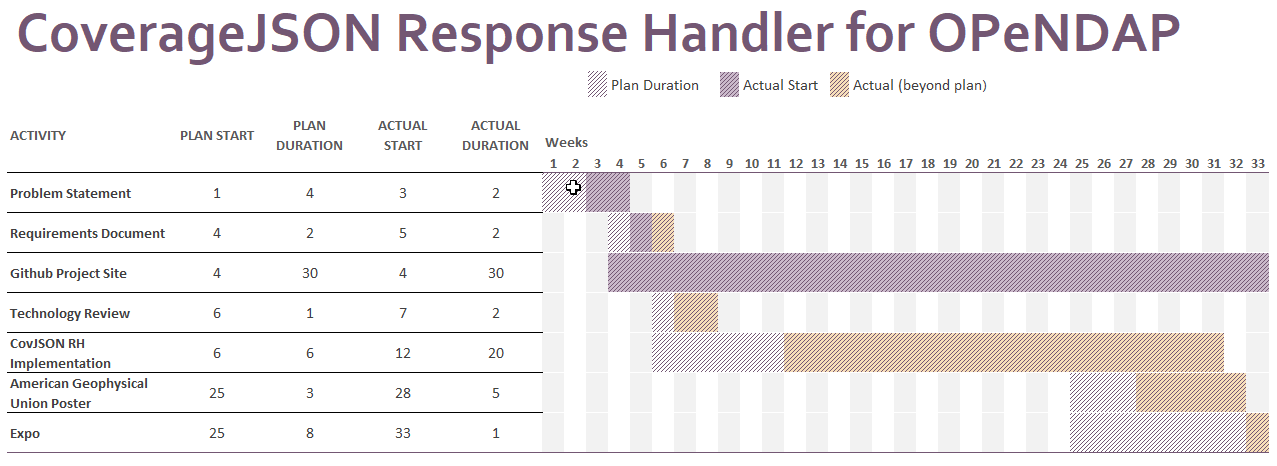
\includegraphics[width=\textwidth]{CS461_Gantt.png}

\subsection{Definitions}
\begin{enumerate}
\item OPeNDAP - Open Source Project for a Network Data Access Protocol
\item CoverageJSON - JSON data format for encoding coverage data
\item JSON - JavaScript Object Notation
\item NASA JPL - The National Aeronautics and Space Administration Jet Propulsion Laboratory
\item Response Handler - the closure that is executed to parse the HTTP response that is returned from the server
\end{enumerate}

\subsection{References}
\begin{enumerate}
\item OPeNDAP Advanced Software for Remote Data Retrieval https://www.opendap.org/
\item CoverageJSON https://covjson.org/
\end{enumerate}

%\subsection{Overview}

\section{Overall Description}
\subsection{Product Perspective}
The CoverageJSON response handler will be incorporated into the larger OPeNDAP open-source software project. Therefore, all function calls will be similar to those implemented in OPeNDAP. The current OPeNDAP JavaScript call looks like this: 
\\\\
\texttt{createDataRequestForm({"url" : "http://test.com/data.gz", "containerID" : "requestform"});}
\\\\The CoverageJSON handler will be similar in execution to remain faithful to the requirements set by OPeNDAP. 

\subsection{Product Functionality}
The CoverageJSON response handler will have the same functionality as the response handlers already implemented in OPeNDAP.
\begin{enumerate}
\item Data that is converted to CovJSON will contain the same information as the source, but in the CovJSON format. 
\item Users will be able to obtain data via a GUI that is already implemented in OPeNDAP, however, there will be a new option for CovJSON.
\item The CovJSON response handler will be integrated into OPeNDAP's source Github. 
\end{enumerate}

\subsection{User Characteristics}
The expected characteristics of a user of the CovJSON response handler will be the same as the characteristics of an expected OPeNDAP user. These characteristics include the following:
\begin{enumerate}
\item Scientists looking to share coverage data over the Internet.
\item Groups looking to provide compatible clients, servers, and SDKs.
\item Users looking to conform to the NASA community standard.

\end{enumerate}
%\subsection{Constraints}

\subsection{Assumptions and Dependencies}
\begin{enumerate}
\item There will be an adequate amount of accurate documentation on OPeNDAP and its response handlers.
\item There will be a Hyrax server environment capable enough to test on.
\item There will be feedback on the testing and documentation needed to have the response handler pulled into the OPeNDAP project.
\end{enumerate}

\section{Requirements}
The CoverageJSON response handler will need to fulfill the following requirements:
\begin{enumerate}
\item Handle and feed out data in the CoverageJSON format.
\item All handled data should match the original source data exactly.
\item Able to be pulled into the OPeNDAP source project.
\item The handler will need to be able to be called in the same fashion that the current OPeNDAP handlers are called, and should behave similarly.
\item The handler must be fully testable and should meet the standards defined by the client.
\item All code should adhere to strict coding standards defined by the client.
\end{enumerate}

\end{document}
